\documentclass{article}
\usepackage[margin=1in]{geometry}
\usepackage{amsmath}
\usepackage{listings}
\usepackage{graphicx}
\usepackage{hyperref}
\usepackage[table]{xcolor} % For coloring tables
\usepackage{array} % For custom column widths
\usepackage{calc} % For calculating widths
\usepackage{float}

\graphicspath{ {./images/} }
\setlength{\parindent}{0pt}

\title{CSP to solve Sudoku}
\author{
\begin{tabular}{rl}
    Abdullah Elsayed Ahmed & 7459\\
    Mohammad Ashraf Hamdy & 7508\\
    Samah Abdelaziz Draz & 7889
\end{tabular}    
}

\date{April 27, 2024}

\begin{document}
\maketitle
\tableofcontents

\section{Introduction}
This is basic Sudoku game with 3 modes.
\begin{figure}[H]
    \centering
    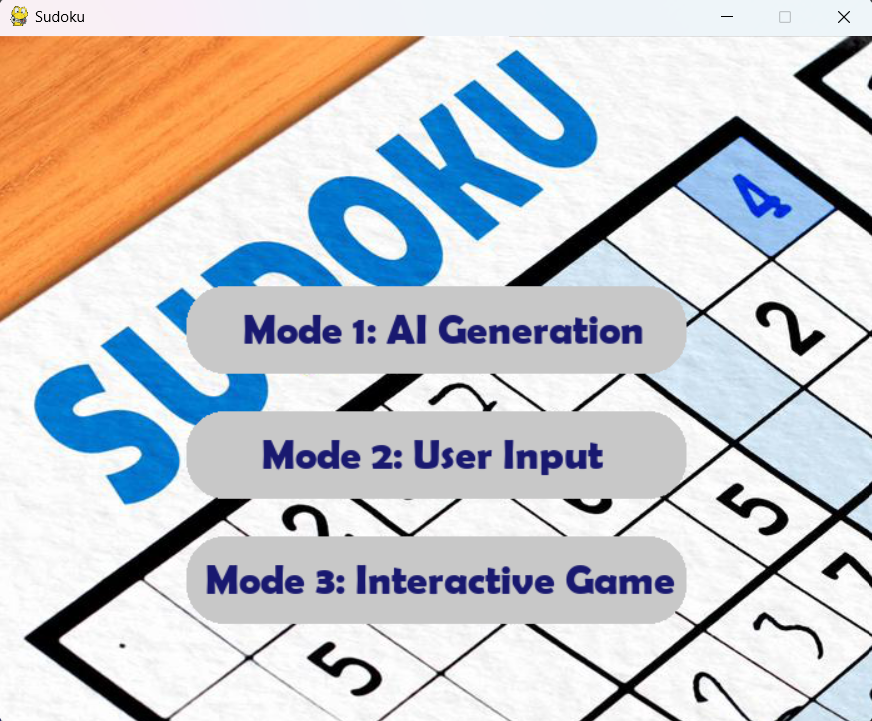
\includegraphics[width=0.7\linewidth]{GUI.png}
    \caption{Sudoku game GUI}
\end{figure}
\section{Data structure}
\subsection*{Array}
Used to represent Sudoku board.
\subsection*{Hast table}
Used to represent the domain of each cell.
\subsection*{Domain}
Used to represent a single cell domain.
\subsection*{Queue}
Used to represent the arcs.


\section{Results}
\subsection*{Easy}
\begin{center}
    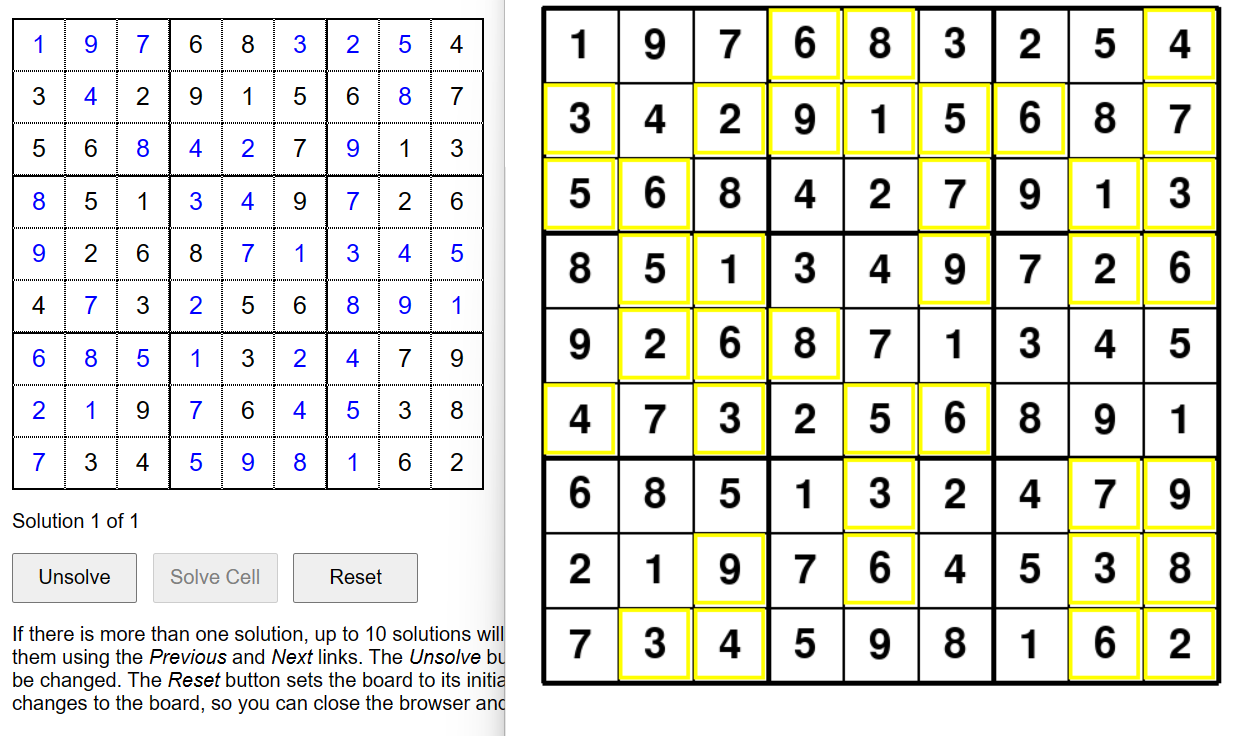
\includegraphics[width=0.8\linewidth]{easy.png}
    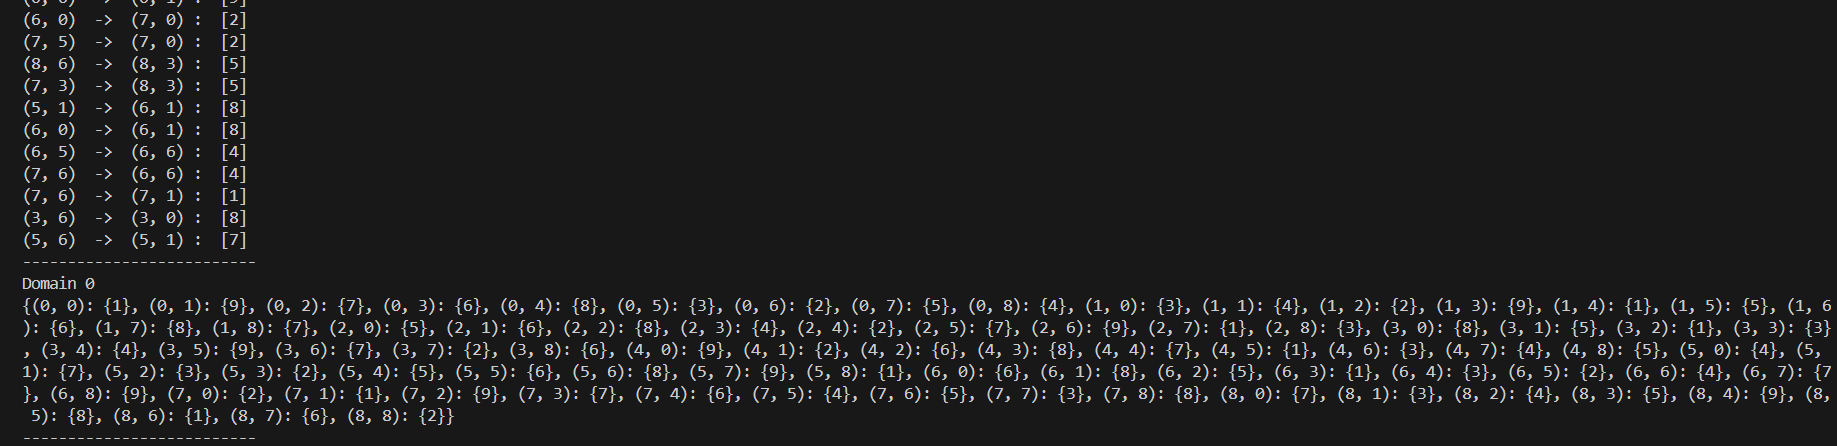
\includegraphics[width=0.8\linewidth]{easy_sample.png}
\end{center}
\begin{itemize}
    \item Time: 0.0033524036407470703
\end{itemize}
\subsection*{Medium}
\begin{center}
    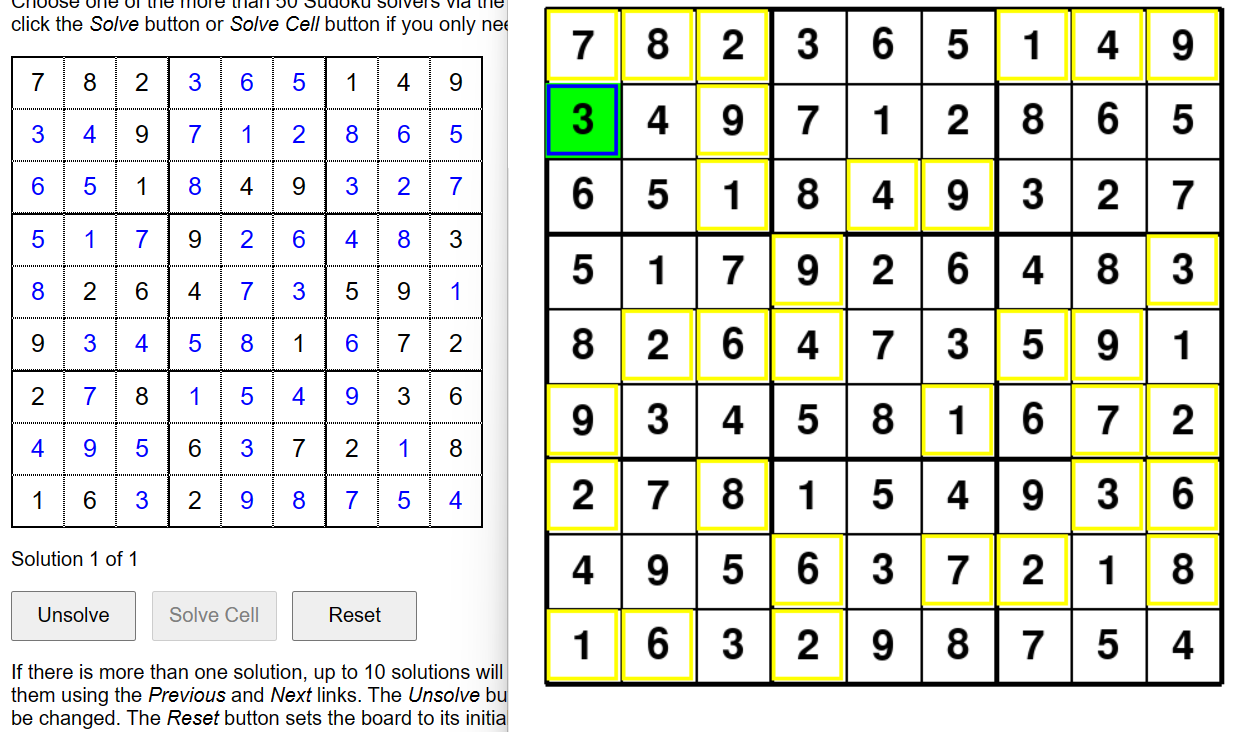
\includegraphics[width=0.8\linewidth]{Medium.png}
    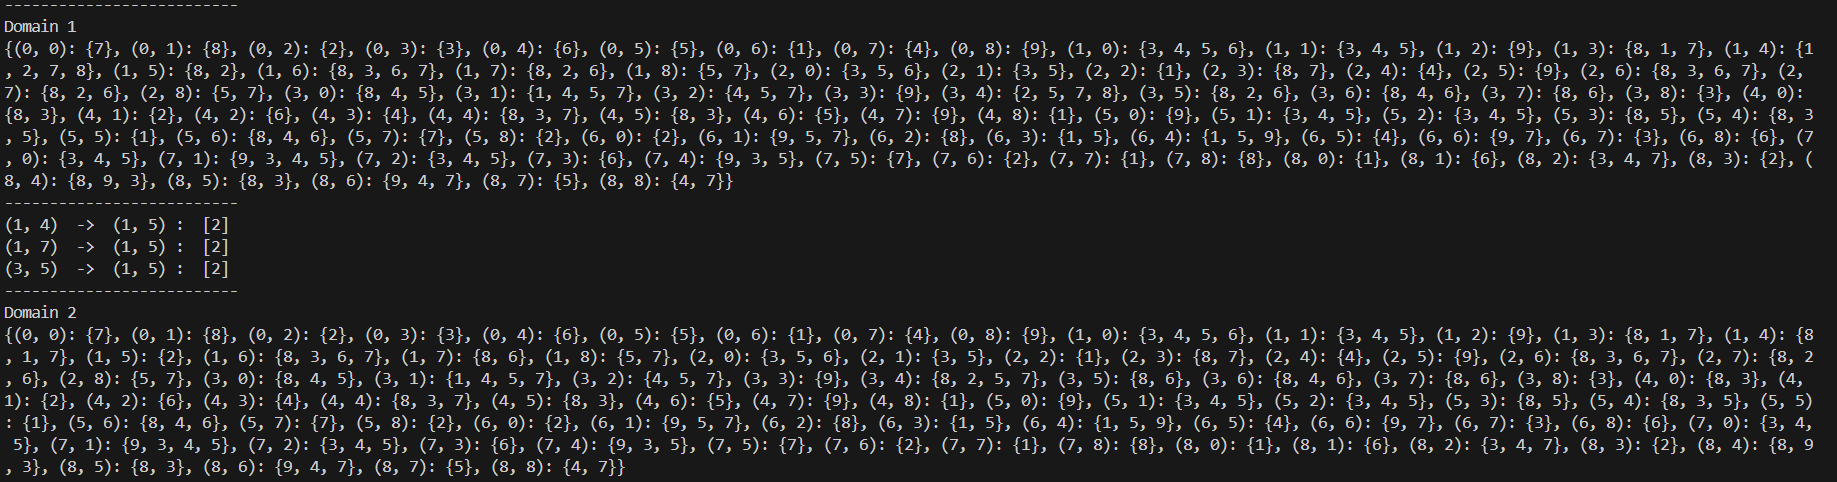
\includegraphics[width=0.8\linewidth]{Medium_sample.png}
\end{center}
\begin{itemize}
    \item Time: 0.006730318069458008
\end{itemize}
\subsection*{Hard}
\begin{center}
    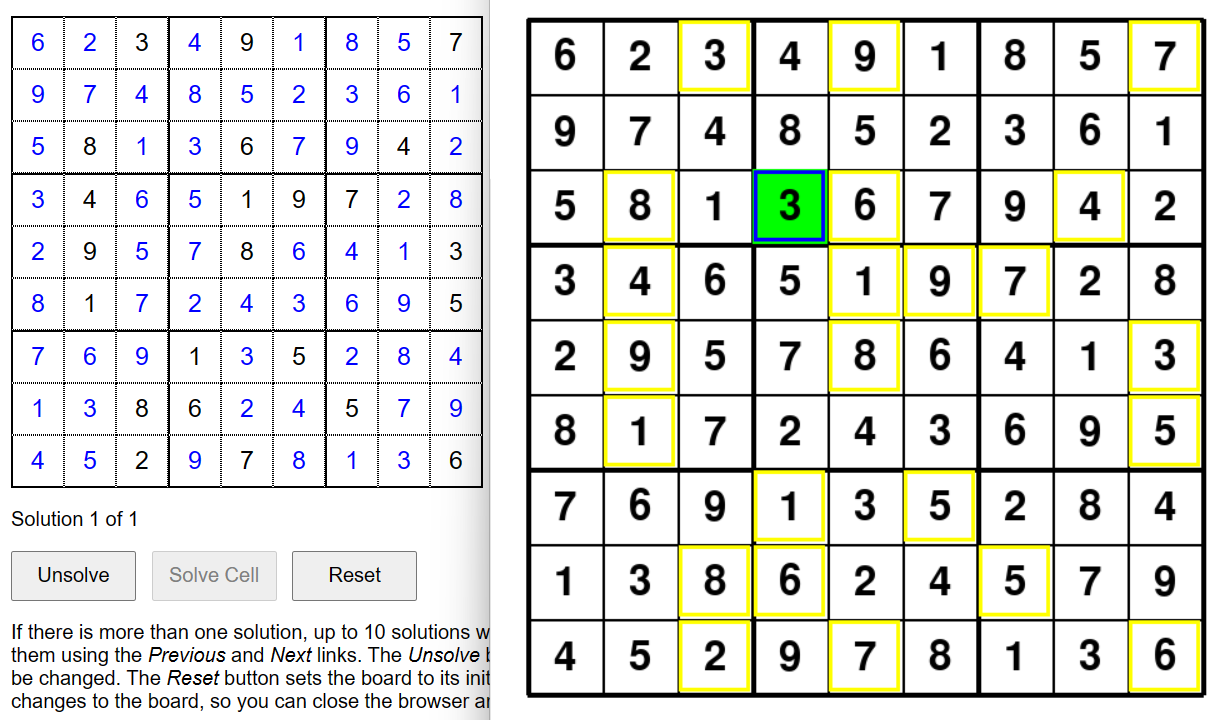
\includegraphics[width=0.8\linewidth]{VeryHard.png}
    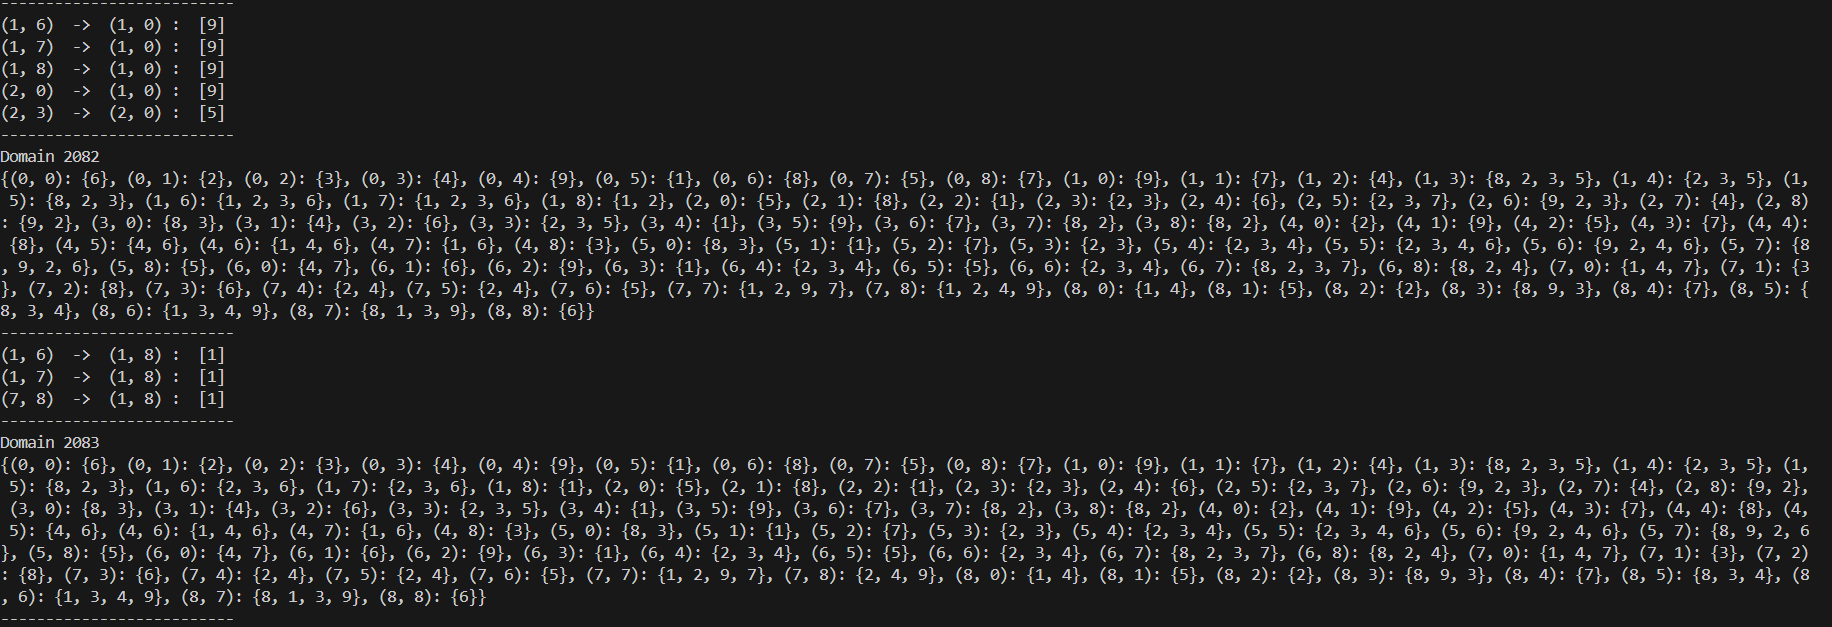
\includegraphics[width=0.8\linewidth]{VeryHard_sample.png}
\end{center}
\begin{itemize}
    \item Time: 0.0128
\end{itemize}

% those are the result of our code each run shows the game board and corresponding minimax trees.
% \subsection*{at k = 1}
% \subsubsection*{Normal minimax}
% \begin{center}
%     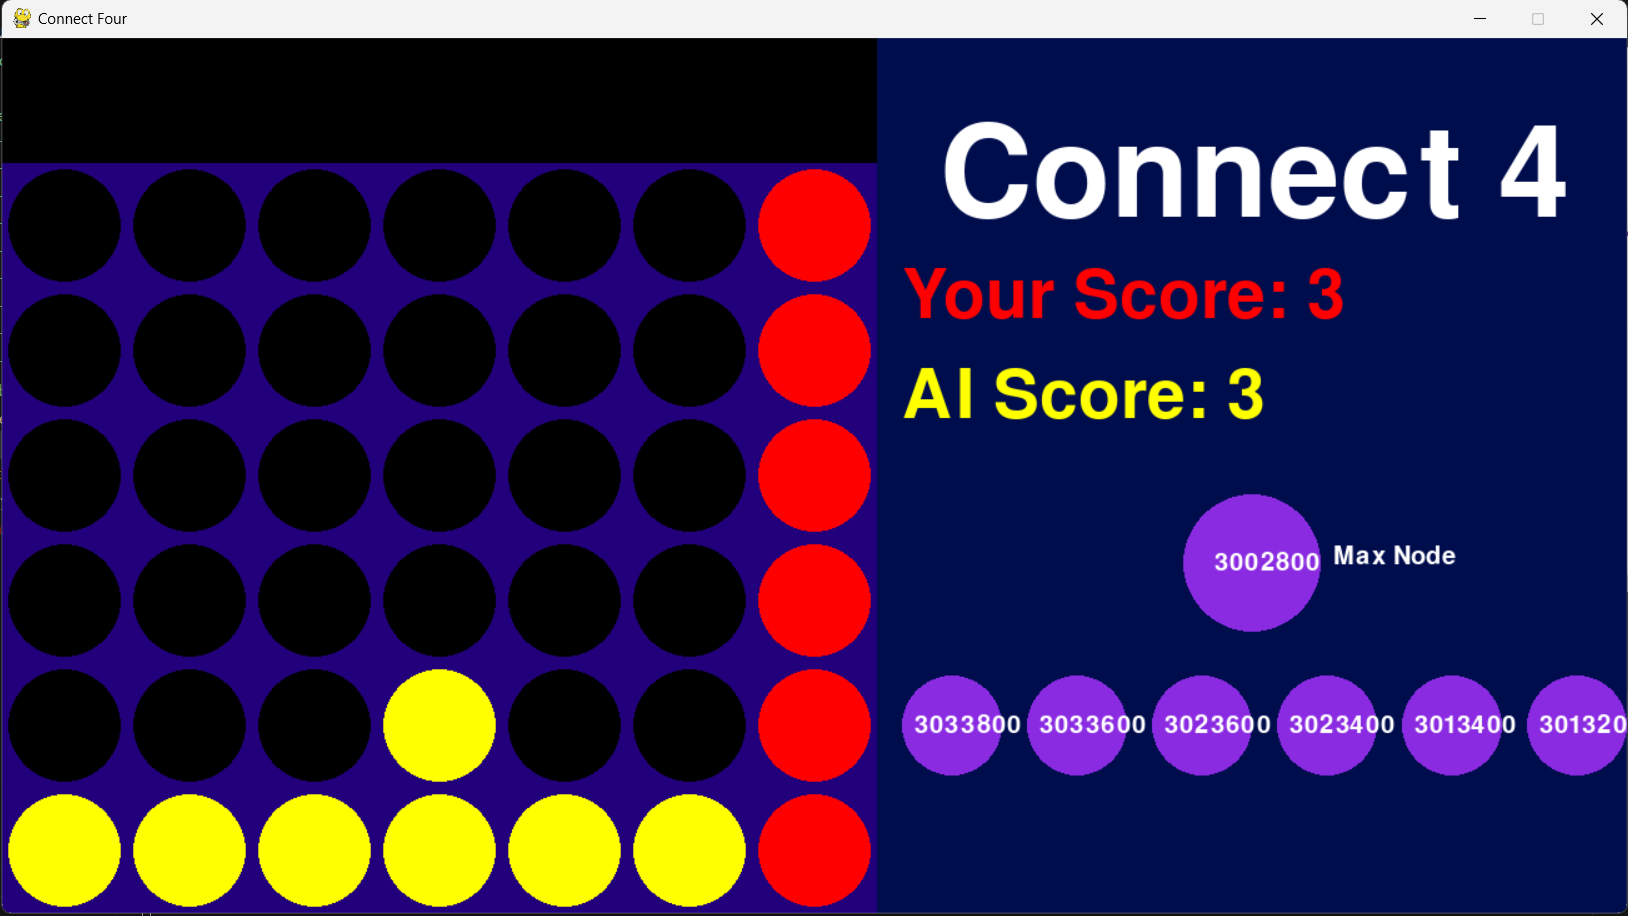
\includegraphics[width=0.8\linewidth]{testcase.png}
% \end{center}
% \begin{itemize}
%     \item Nodes: 48
%     \item Time: 0.004051923751831055
% \end{itemize}
% \subsubsection*{Pruning minimax}
% \begin{center}
%     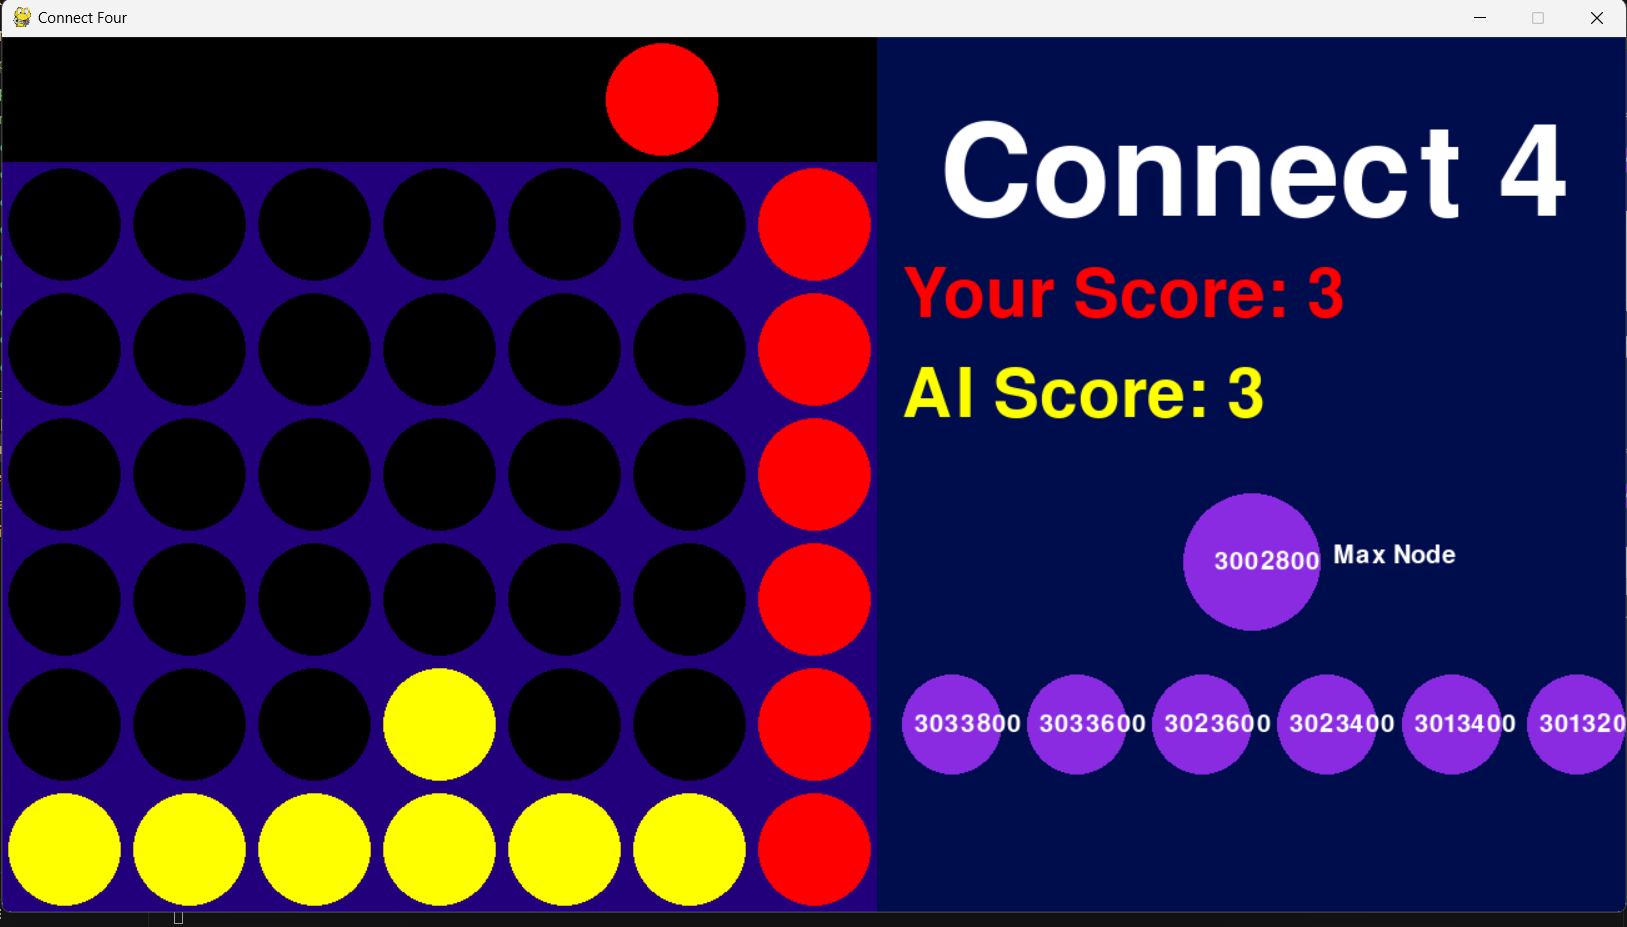
\includegraphics[width=0.8\linewidth]{pruning1.png}
% \end{center}
% \begin{itemize}
%     \item Nodes: 48
%     \item Time: 0.0041010379791259766
% \end{itemize}
% \subsubsection*{Expectation minimax}
% \begin{center}
%     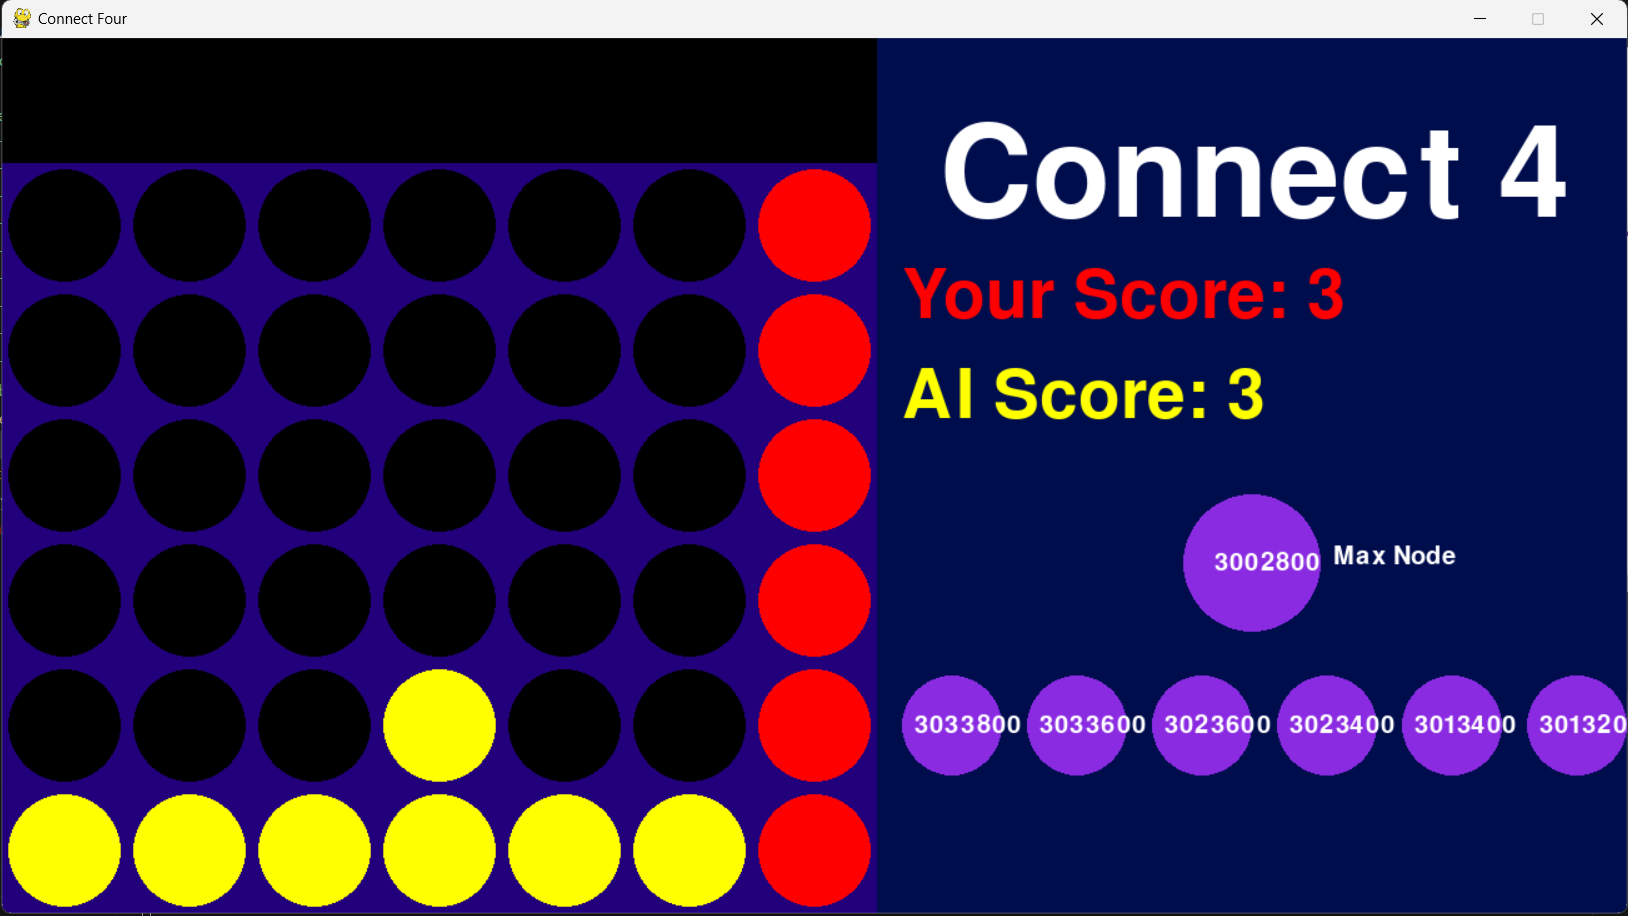
\includegraphics[width=0.8\linewidth]{testcase.png}
% \end{center}
% \begin{itemize}
%     \item Nodes: 48
%     \item Time: 0.003995418548583984
% \end{itemize}
% \subsection*{at k = 3}
% \subsubsection*{Normal minimax}
% \begin{center}
%     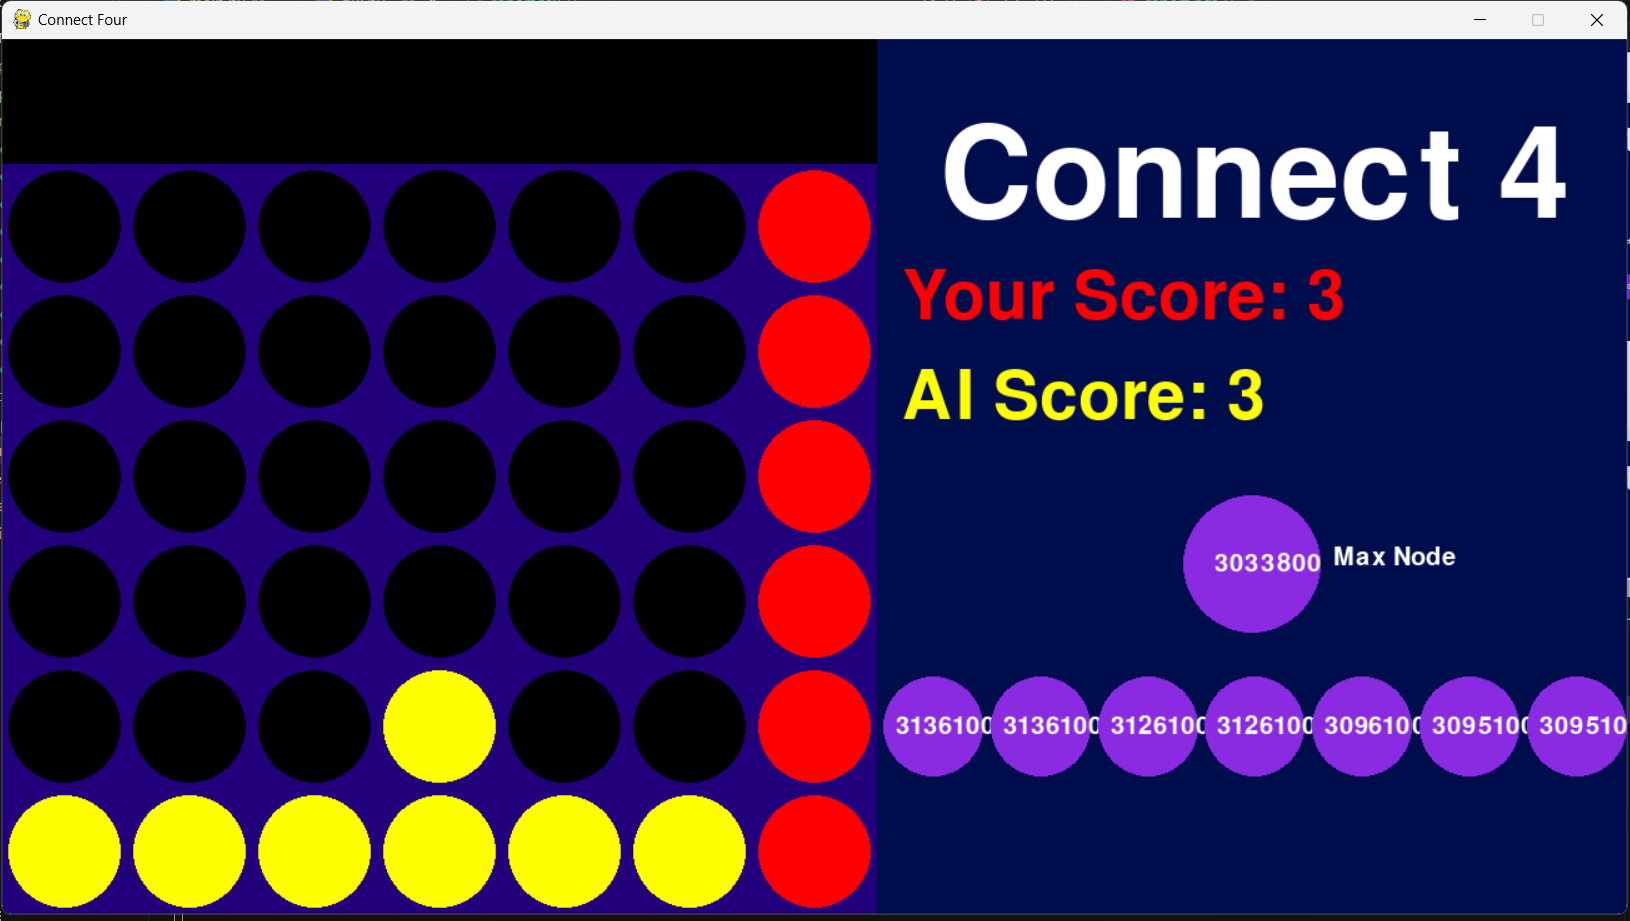
\includegraphics[width=0.8\linewidth]{testcase3.png}
% \end{center}
% \begin{itemize}
%     \item Nodes: 2631
%     \item Time: 0.12168431282043457
% \end{itemize}
% \subsubsection*{Pruning minimax}
% \begin{center}
%     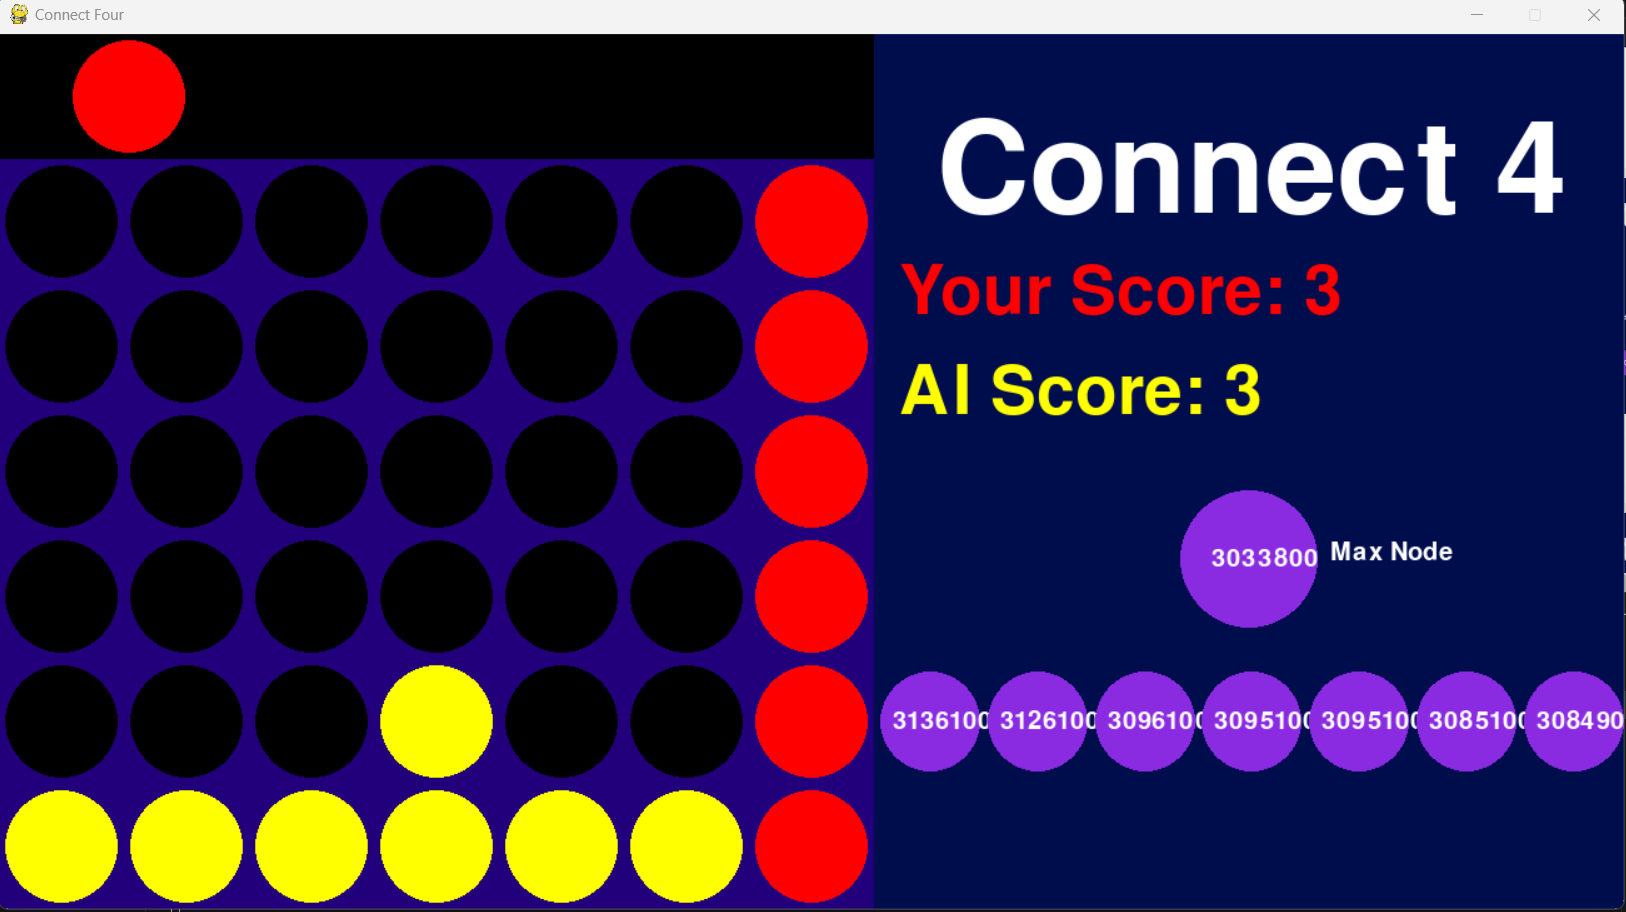
\includegraphics[width=0.8\linewidth]{pruning3.png}
% \end{center}
% \begin{itemize}
%     \item Nodes: 1056
%     \item Time: 0.04659581184387207
% \end{itemize}
% \subsubsection*{Expectation minimax}
% \begin{center}
%     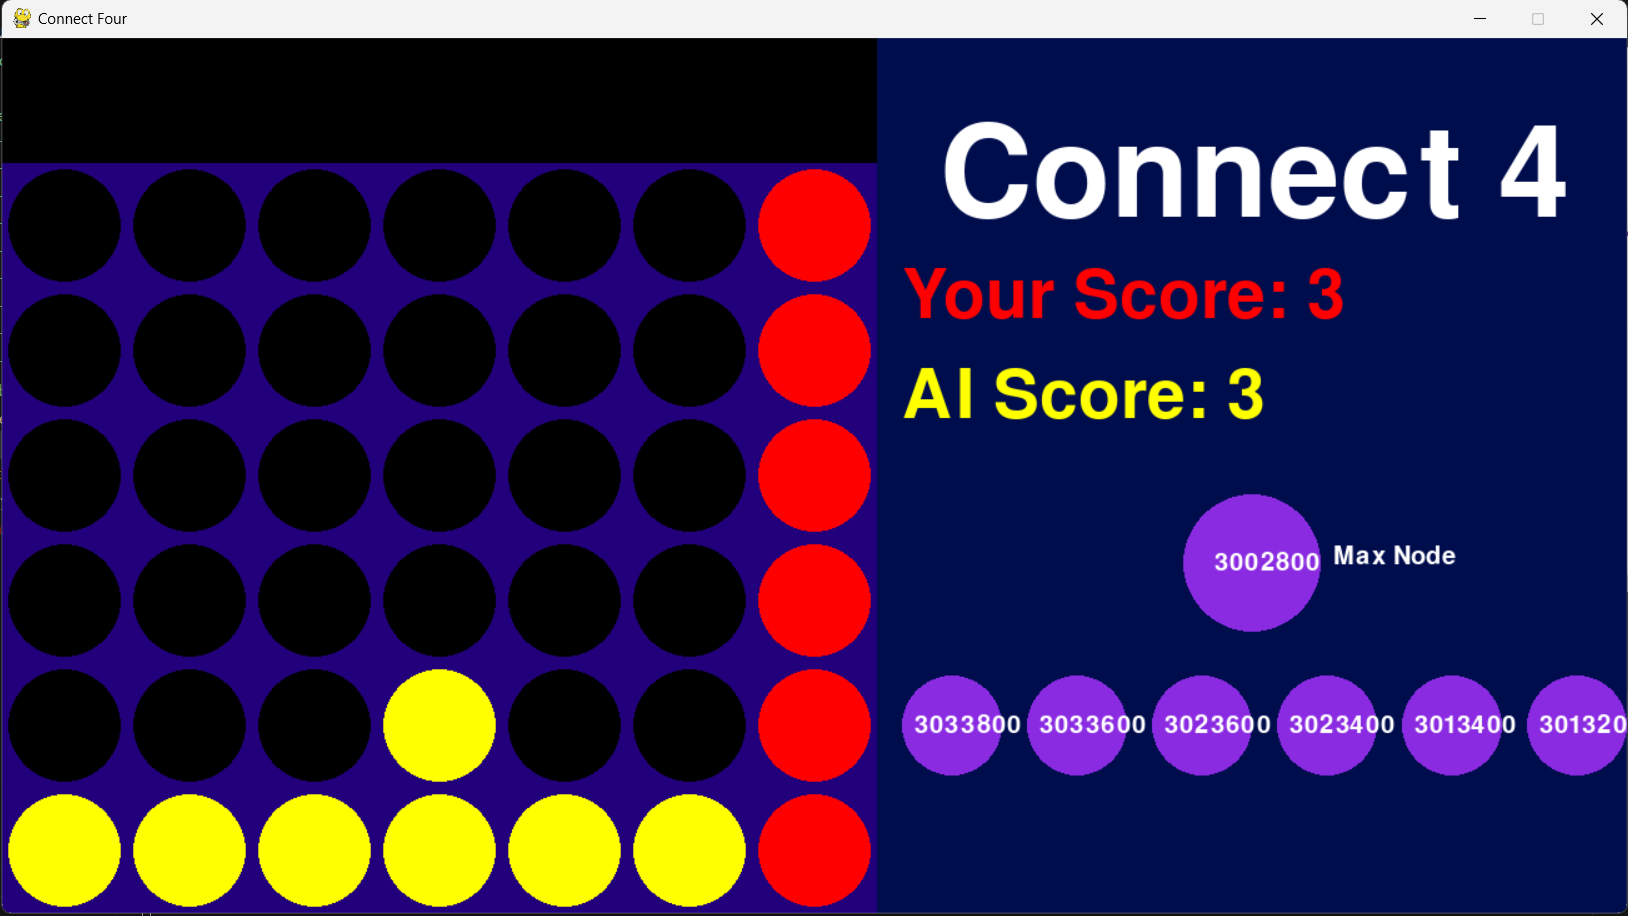
\includegraphics[width=0.8\linewidth]{testcase.png}
% \end{center}
% \begin{itemize}
%     \item Nodes: 1056
%     \item Time: 0.04659581184387207
% \end{itemize}
% \subsection*{at k = 5}
% \subsubsection*{Normal minimax}
% \begin{center}
%     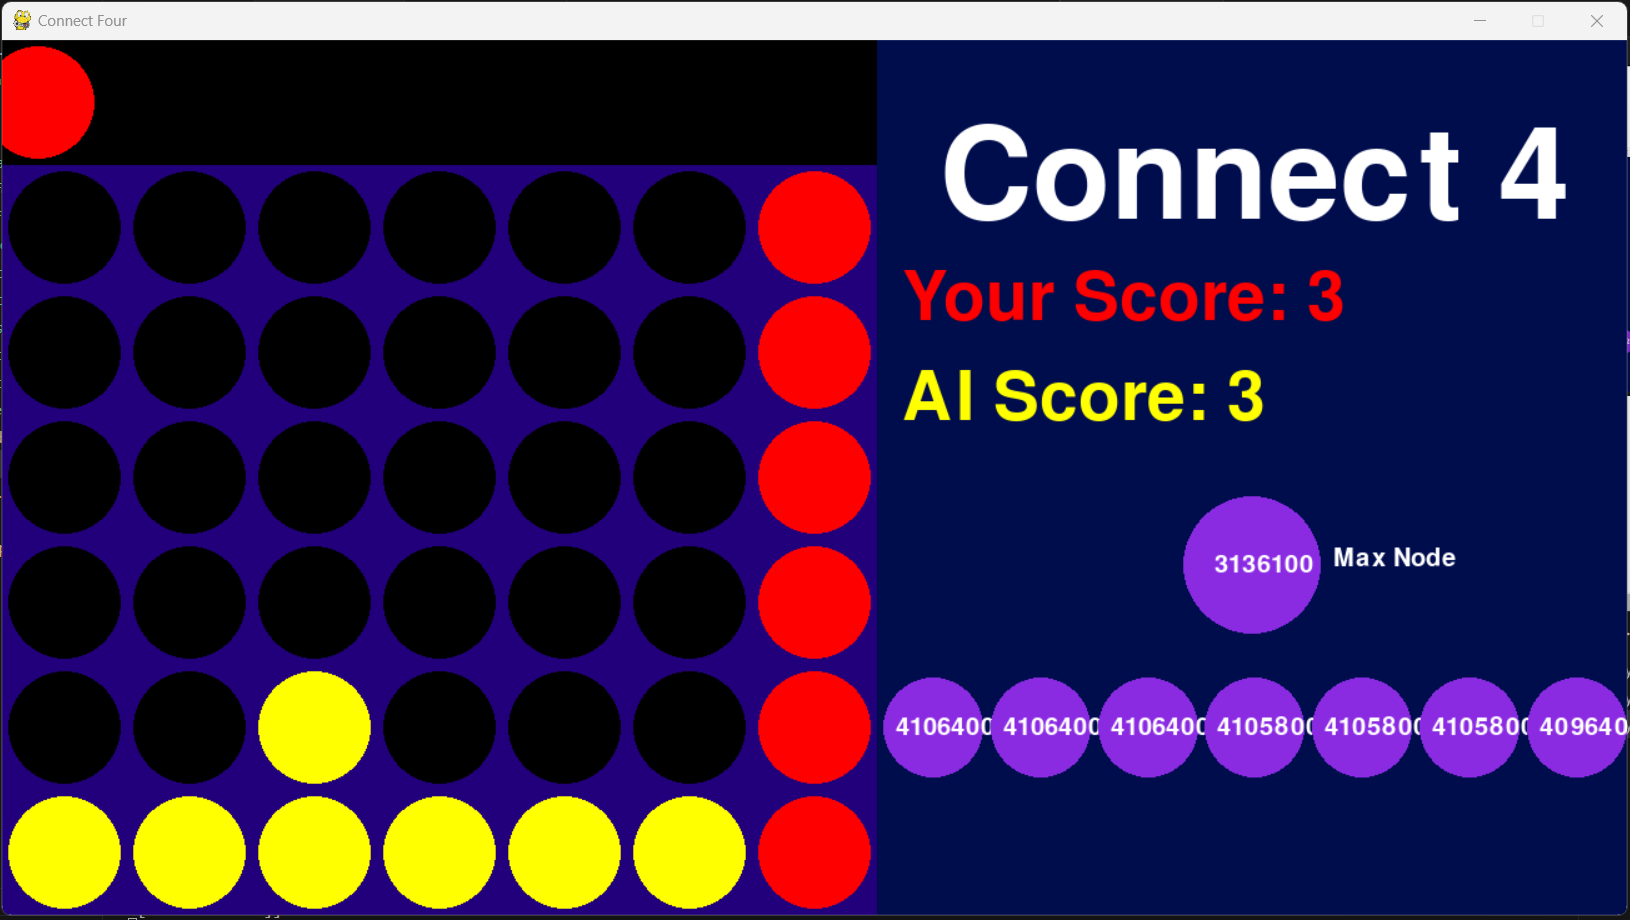
\includegraphics[width=0.8\linewidth]{testcase5.png}
% \end{center}
% \begin{itemize}
%     \item Nodes: 62621
%     \item Time: 1.756775140762329
% \end{itemize}
% \subsubsection*{Pruning minimax}
% \begin{center}
%     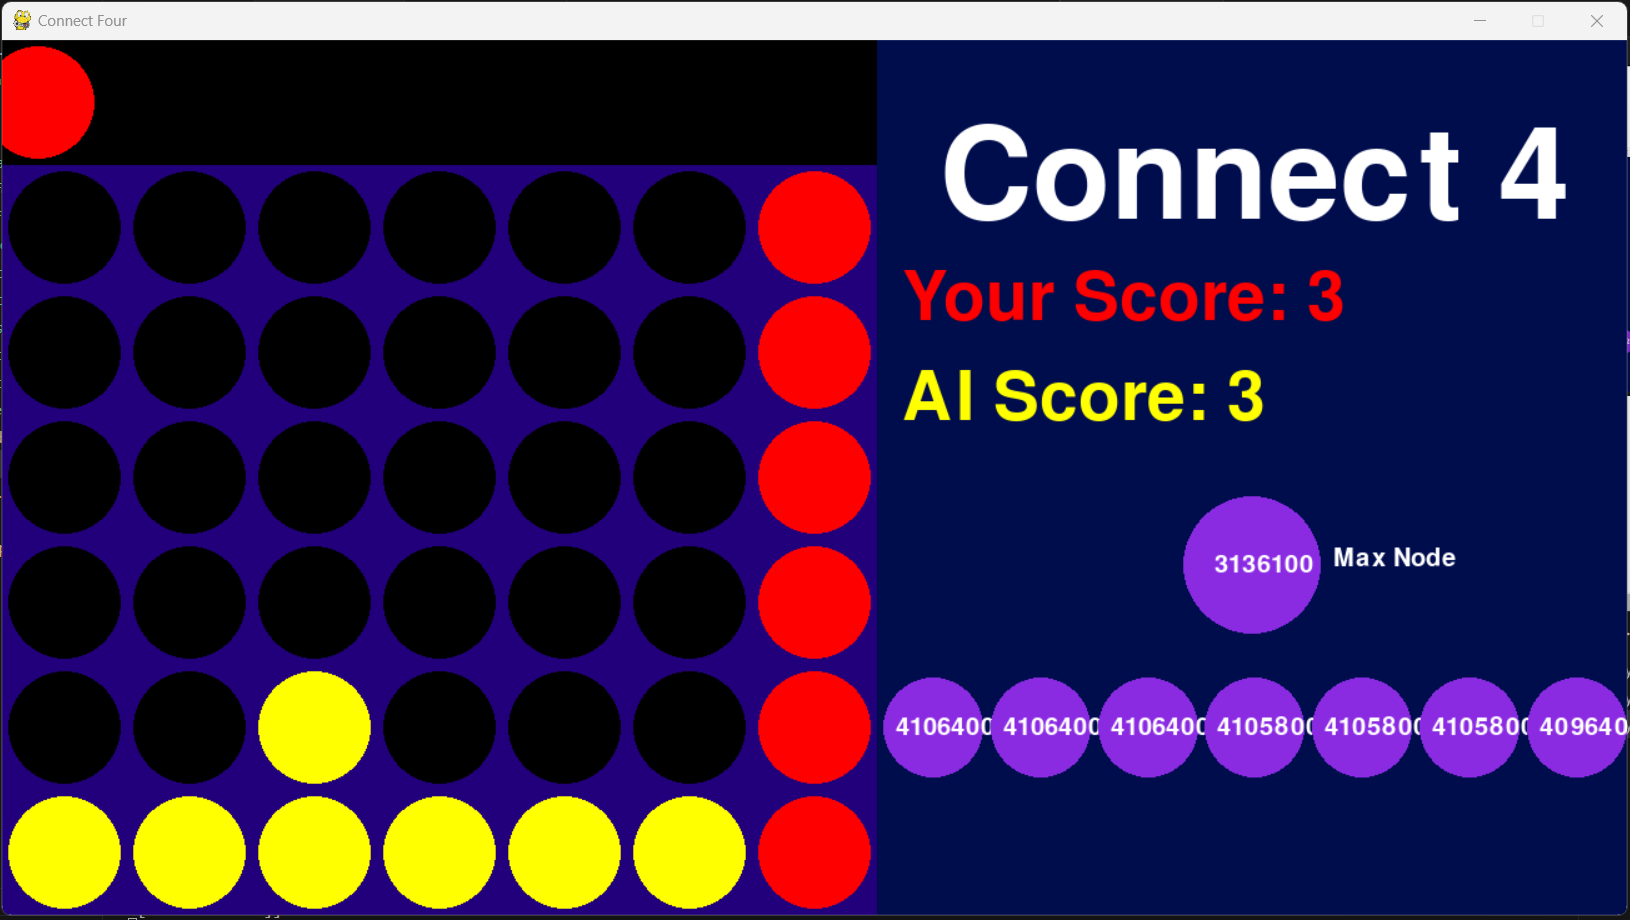
\includegraphics[width=0.8\linewidth]{pruning4.png}
% \end{center}
% \begin{itemize}
%     \item Nodes: 11710
%     \item Time: 0.6393032073974609
% \end{itemize}
% \subsubsection*{Expectation minimax}
% \begin{center}
%     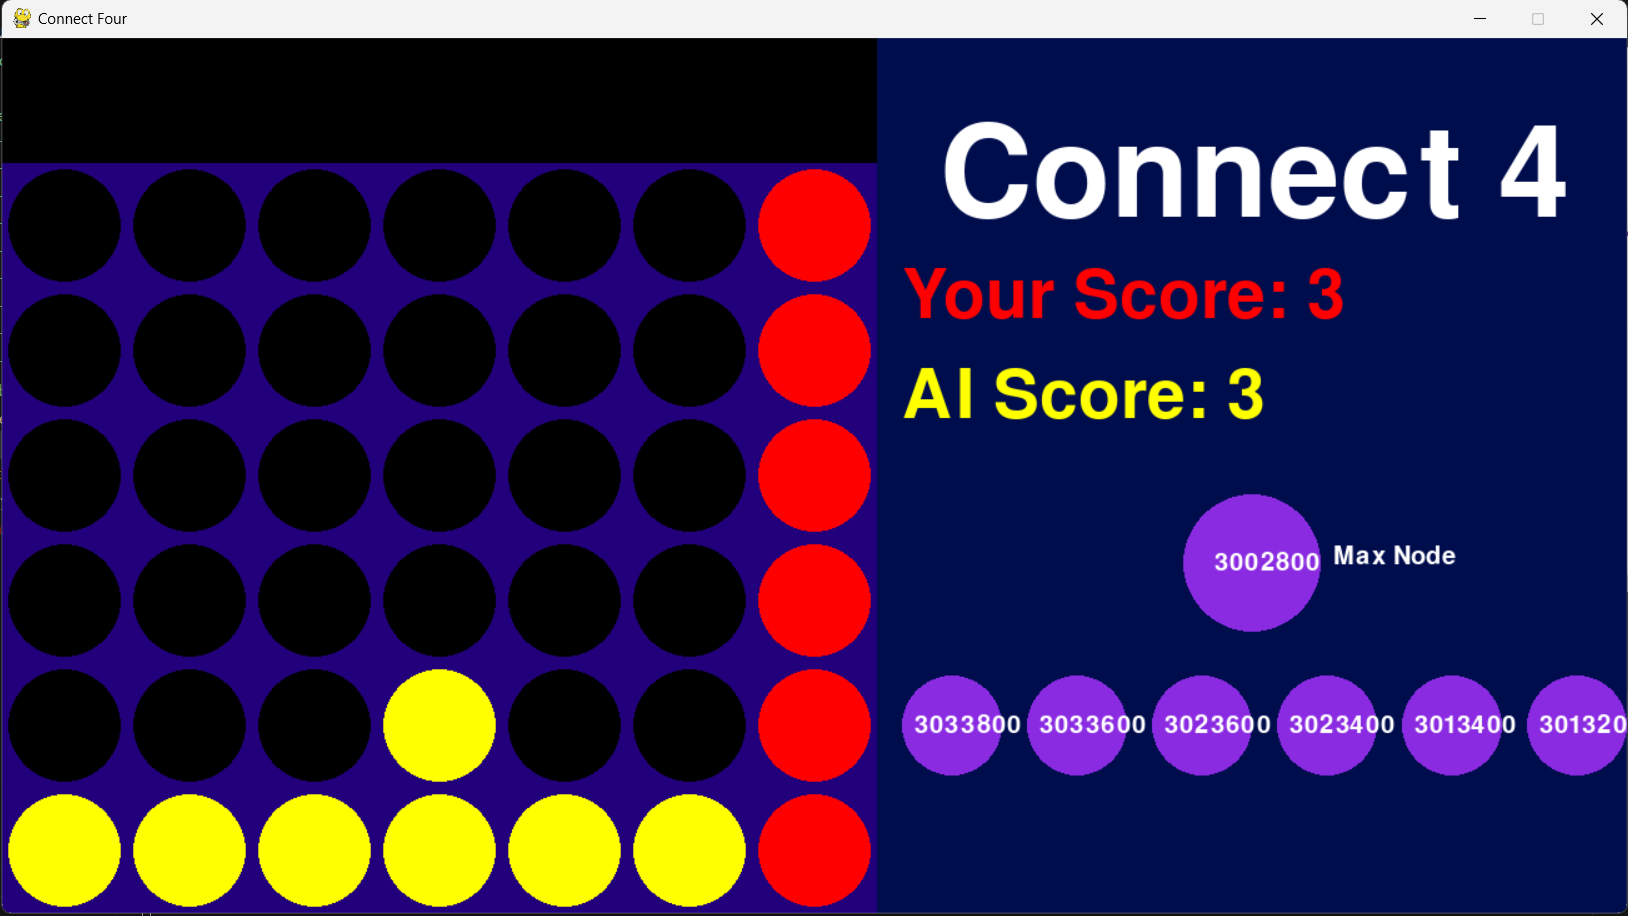
\includegraphics[width=0.8\linewidth]{testcase.png}
% \end{center}
% \begin{itemize}
%     \item Nodes: 11710
%     \item Time: 0.6393032073974609
% \end{itemize}
\newpage
\section{Conclusion}
From our result we can compare different minimax approach at different K values.

% \subsection*{at K = 1}
% \subsubsection*{Normal minimax}
% \subsubsection*{Pruning minimax}
% \subsubsection*{Expectation minimax}
% \subsection*{at K = 3}
% \subsubsection*{Normal minimax}
% \subsubsection*{Pruning minimax}
% \subsubsection*{Expectation minimax}
% \subsection*{at K = 5}
% \subsubsection*{Normal minimax}
% \subsubsection*{Pruning minimax}
% \subsubsection*{Expectation minimax}
\subsection*{In General}
\subsubsection*{Normal minimax}
It is the worst of them because It has to check losing move also it is not important no more (due to a better move is available).
\subsubsection*{Pruning minimax}
It is better version of normal minimax (minimax without alpha beta Pruning) due to the pruning process.
\subsubsection*{Expectation minimax}
It is slightly better then Pruning minimax.

\end{document}